

In this chapter we provide the expressions of the closure terms of a dilute and viscous dominated regime emulsion of spherical droplets. 
% We will consider a monodisperse suspension of droplets with radius $a$ and constant viscosity $\lambda \mu_f$. 
It must be understood that our goal is not to derive a set of equations for non-inertial spherical particles, in which case the energy equations and first-order moment equations would be unnecessary. 
Instead, we provide the closures in the limit of Stokes flow regime to illustrate their physical implication. 
% Thus, even though the closures are expressed in the Stokes limit, note that the set of equations provided remains valid regardless of the flow regime.

\section{Derivation of the closure terms for dilute emulsion of spherical droplets in Stokes flows}
\label{sec:application}

% \subsection{Discussion of the closures }




The closure terms presented in this section are based on the singularity solution of an isolated droplet in a linear flow. 
For illustrating purposes, we displayed on \ref{fig:flowlines} the flow lines of these solutions, both uniform flow and linear flow. 
More details on the computation of these singularity solutions are given in \ref{ap:solution_singularity}. 
Note that a quadratic background flow contribution could be taken into account since the solution is known \citep{nadim1991motion}, nevertheless it is not considered here for simplicity. 
\begin{figure}[h!]
    \centering
    \begin{tikzpicture}
        % \node (img3) at (0.6\textwidth,0) {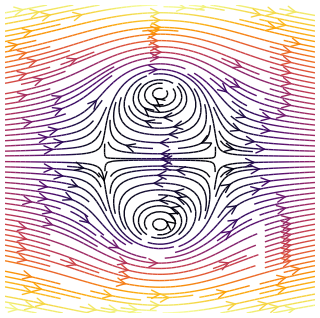
\includegraphics[width=0.3\textwidth,angle=270]{image/Rising_def_Stokes.png}};
        \node (img2) at (0.0\textwidth,0) {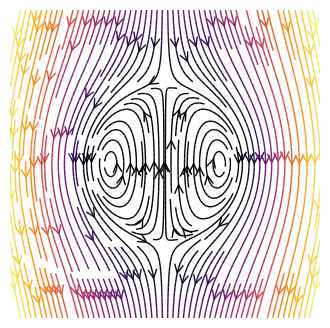
\includegraphics[width=0.3\textwidth]{image/Rising_Stokes.png}};
        \node (img1) at (0.3\textwidth,0) {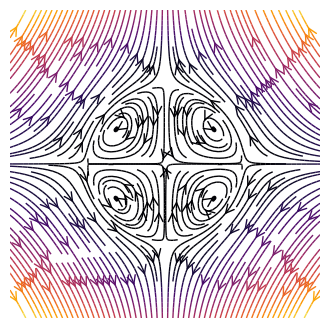
\includegraphics[width=0.3\textwidth]{image/Shear_Stokes.png}};
        % \draw (0.45\textwidth,0)node{$\rightarrow$};
        % \draw (0.45\textwidth,0.4cm)node{$\bm\Gamma_\alpha\cdot \textbf{r}$};
        % \draw (img3.south)node{(c)};
        \draw (img2.south)node{(a)};
        \draw (img1.south)node{(b)};
    \end{tikzpicture}
    \caption{Examples of steady state flow lines plots of an isolated droplet immersed into a viscous fluid. 
    (a) Rising sphere in uniform stokes flow. 
    (b) Fixed droplet in a pure extensional.
    (analytical solution in \ref{ap:solution_singularity})
    These solutions correspond exactly to the fields $\textbf{u}_f^1$ at order $\mathcal{O}(\phi_d)$.}
    % (c) Deformed droplet in rising motion (analytical solution of \citet{taylor1964deformation}). }
    \label{fig:flowlines}
\end{figure}

We recall that all along this section we consider spherical droplets of radius $a$ with viscosity ratio $\lambda = \mu_d /\mu_f$ and density ratio $\zeta =\rho_d /\rho_f$. 
Thus the problem \ref{eq:conditional_avg_eq_final_stokes} can be easily solved and have the solutions, 
\begin{align}
    \label{eq:singularity_solution_out}
    \textbf{u}_\text{out}^{1d}[\textbf{r},\textbf{w}]
    &= 
    \mathcal{U}_\text{out}[\textbf{r}] \cdot \textbf{u}_{fw}
    + \mathcal{E}_\text{out}[\textbf{r}]: \textbf{E}_{f}\\
    \textbf{u}_\text{in}^{1d}[\textbf{r},\textbf{w}]
    &= 
    \mathcal{U}_\text{in}[\textbf{r}] \cdot \textbf{u}_{fw}
    + \mathcal{E}_\text{in}[\textbf{r}] : \textbf{E}_{f}
    \label{eq:singularity_solution_in}
\end{align}
where $\textbf{r} = \textbf{x} - \textbf{y}$, $\textbf{u}_{fw} = \textbf{u}_f - \textbf{w}$, the subscript ``in'' indicates that the solution is valid inside the domain $|\textbf{r}| <1$, and the subscript ``out'' in $|\textbf{r}|>1$. 
$\textbf{E}_f = \grad \textbf{u}_f + (\grad \textbf{u}_f)^\dagger$ is the mean shear rate tensor of the continuous phase. 
Note that at first order in $\phi_d$, $\phi_d\textbf{u}_f =\phi_d\textbf{u} - \phi_d^2 \textbf{u}_d = \phi_d\textbf{u}$, so one can either use $\textbf{u}_f$ or $\textbf{u}$ in the above definition of $\textbf{u}_{fw}$. 
The second and third order tensor $\mathcal{U}_\text{out},\mathcal{U}_\text{in},\mathcal{E}_\text{out}$ and $\mathcal{E}_\text{in}$ read as, 
\begin{align}
    (\mathcal{U}_{\text{out}})_{ik} &= 
    \frac{1}{4}\left(\frac{3\lambda + 2}{\lambda +1}\right)
    \left(\frac{\delta_{ik}}{r} + \frac{r_ir_k}{r^3}\right) 
    + 
    \frac{1}{4}\left(\frac{\lambda}{\lambda +1}\right)
    \left(\frac{\delta_{ik}}{r^3} - \frac{3r_ir_k}{r^5}\right),  \\
    (\mathcal{E}_{\text{out}})_{ijk}
    &=
    %  \bm\delta\textbf{r}
    -\frac{\lambda}{(\lambda + 1)r^5} \delta_{ij}r_k
    -\left(\frac{5\lambda +2}{2(\lambda +1 )r^5} - \frac{5\lambda}{2(\lambda+1)r^7}\right) r_ir_jr_k,\\
    (\mathcal{U}_\text{in})_{ik}  &= 
    \frac{1}{2}\left(\frac{2\lambda +3}{\lambda +1}\right)\delta_{ik}
    -\frac{1}{2} (2r^2 \delta_{ik} - r_ir_k)
    \left(\frac{1}{\lambda +1}\right),\\
    (\mathcal{E}_\text{in})_{ijk}
    &=
    \frac{5r^2 -3}{2(\lambda +1)} r_i\delta_{jk}
    - \frac{1}{\lambda+1}r_ir_jr_k. 
\end{align}
Note that we did not consider the rotation of the particles nor the mean vorticity of the flow. 
This is because we consider ``torque free'' droplets, which implies that they follow the continuous phase vorticity and do not generate disturbance. 
Hence, none of the closure terms will be impacted by the rotation of droplets. 

\subsection{Moment of force traction}

Let us present in the first place the closures for the momentum exchange term present in \ref{eq:dt_hybrid_rhou_f}. 
Using \ref{eq:singularity_solution_out} and \ref{eq:drag_final2} it is found that the first three moments of the hydrodynamic forces are related to the mean fluid and particle phase velocity field as, 
\begin{align}
    \label{eq:zeroth_mom}
    \pSavg{\bm{\sigma}_f^0\cdot \textbf{n}_d} &= 
    \phi_d \div\bm\Sigma_f
    + \frac{3\phi_d\mu_f}{2 a^2} 
    \left(\frac{3\lambda+2}{\lambda+1}\right) \textbf{u}_{f p} 
    + \frac{3\phi_d\mu_f}{4} \left(\frac{\lambda}{\lambda+1}\right)\grad^2\textbf{u}_f\\
    \label{eq:first_mom}
    \pavg{\intS{\textbf{r}\bm{\sigma}_f^0 \cdot \textbf{n}_d}} 
    &= 
    \phi_d \bm\Sigma_f + 
    \frac{3}{5}\mu_f \phi_d \left(\frac{2+5\lambda}{1+\lambda}\right)
    \textbf{E}_f
    \\
    \label{eq:second_mom}
        \pavg{\intS{(\bm{\sigma}_f^0 \cdot \textbf{n}_d)_ir_kr_l}} &=
        % \phi_d  \frac{a^2}{5} 3 [(\div \bm\Sigma_f)\bm\delta]^\text{sym}
        + \frac{3\mu_f\phi_d}{2}\left(\frac{\lambda}{\lambda+1}\right)(\textbf{u}_{fp})_i\delta_{kl}\\
        &+ \frac{3\mu_f\phi_d}{5}\left(\frac{1}{\lambda+1}\right)((\textbf{u}_{fp})_i\delta_{kl}+ (\textbf{u}_{fp})_k\delta_{il}+(\textbf{u}_{fp})_l\delta_{ki})\nonumber
\end{align}
where we recall that $\textbf{u}_{fp} = \textbf{u}_f - \textbf{u}_p$, $\bm\Sigma_f = -p_f\bm\delta +2 \mu_f \textbf{E}_f$, and $\textbf{E}_f = \frac{1}{2}\left[\grad \textbf{u}_f + (\grad \textbf{u}_f)^\dagger\right]$. 
The term $\pSavg{\bm{\sigma}_f^0 \cdot \textbf{n}_d}$ represents the total components of the interphase force.
Specifically, the first term is the mean Newtonian continuous phase stress $\bm\Sigma_f$, the second term is the Hadamard-Rybczynski force, and the last is the Faxen contribution \citep{kim2013microhydrodynamics}. 
\footnote{Note, that the Faxen contribution cannot be derived directly from \ref{eq:singularity_solution_in} and \ref{eq:singularity_solution_out} since we did not consider quadratic contribution in the background flow.
However it can be obtained with the use of the reciprocal theorem, more details is given in \citet{kim2013microhydrodynamics} or in \ref{ap:reciprocal} where we re-demonstrate the calculation. }
Likewise, $\pSavg{\textbf{r}\bm{\sigma}_f^0 \cdot \textbf{n}_d}$ is the averaged first moment of the surface force traction, which includes the mean fluid phase stress. 
This tensor is responsible for the well-known Einstein correction to the viscosity (see next section), but here it is adapted to spherical droplets instead of spherical solid particles \citep{rallison1978note}. 
The second moment of the force traction is made of two contributions, the first one is related to the divergence of the mean fluid phase stress (not shown here, see \ref{eq:second_mom_general}). 
However, this contribution is negligible at $\mathcal{O}(\phi_d)$ \citep{jackson1997locally} and therefor not shown in \ref{eq:second_mom}.  
The second contribution is proportional to the relative velocity $\textbf{u}_{fp}$.
This term was first discovered by \citet{nozieres1987local} based on phenomenological arguments and by \citet{lhuillier1992volume} based on theoretical ground, both for spherical solid particles. 
According to the cited author, this term induces a coupling between relative motion and convection. 
According to \ref{eq:second_mom} the second moment of the hydrodynamic forces is non-negligible at first order in $\phi_d$, in agreement with \citep{jackson1997locally,zhang1997momentum}. 
Thus, the zeroth, first, and second moment of the drag are non-negligible in the Stokes regime and at $\mathcal{O}(\phi_d)$. 
In \citet{zhang1997momentum} they even stipulated that the third order moment of the force traction is not necessarily negligible at $\mathcal{O}(\phi_d)$ when considering non-spherical particles in stokes flows. 

Consequently, in the Stokes and dilute hypothesis, the zeroth, first, and second moments of surface traction are non-negligible and are primordial in the modeling of the fluid phase momentum equations. 
These terms might be also relevant for broader flows regimes. 
For example, in \ref{chap:deformable} we demonstrate that \ref{eq:first_mom} has a component proportional to the mean phase velocity $\textbf{u}_{fp}\textbf{u}_{fp}$ at low but finite inertial regime. 
Thus, it is surprising that most studies in the literature do not mention the first and second-order moments, which are almost always neglected. 

\subsection{Pseudo turbulent stress tensor}

Another contribution to the effective stress is the pseudo-turbulent tensor $\avg{\chi_f \textbf{u}_f'\textbf{u}_f'}$ (see \ref{eq:sigma_eq_def}). 
Note that in the Stokes regime this term is more likely to be negligible, nevertheless, it is still interesting to provide its closure based on the Stokes flow problem, as it results in the first-order closure in $Re$, which is relevant for finite particle Reynolds number flows.

This closure term can be computed based on \ref{eq:Batchelor2}. 
Indeed, according to \ref{eq:Batchelor2} we may reformulate $\avg{\chi_f \textbf{u}_f'\textbf{u}_f'}$ in terms of an integral of $\textbf{u}_\text{out}^{1d}\textbf{u}_\text{out}^{1d}$ over $\textbf{w}$ and $\textbf{x}$. 
In the Stokes regime $\textbf{u}_\text{out}^{1d}$ is proportional to $\textbf{u}_{fw} = \textbf{u}_f - \textbf{w}$ and $\textbf{E}_f$, see \ref{eq:singularity_solution_out}. 
Since, $\avg{\chi_f \textbf{u}_f'\textbf{u}_f'}$ is a symmetric second-order tensor, the final closure must remain symmetric and second-order.
The only possible combination of tensor, $\textbf{u}_{fw}$ and $\textbf{E}_f$, which can form a symmetric second-order tensor are, 
\begin{align}
    \textbf{u}_{fw}
    \textbf{u}_{fw}
    &&
    \textbf{E}_f\cdot \textbf{E}_f
    && 
    (\textbf{u}_{fw}\cdot 
    \textbf{u}_{fw})\bm\delta
    &&
    (\textbf{E}_f : \textbf{E}_f)\bm\delta. 
\end{align}
Note that it is impossible to obtain a second-order tensor based on combination of one vector ($\textbf{u}_{fw}$), and one second-order tensor ($\textbf{E}_f$). 
Therefore, we deduce that at the leading order in Reynolds number and particle volume fraction, the covariance between the disturbance field of a particle in translation (i.e. $\mathcal{U}_\text{out}[\textbf{r}] \cdot \textbf{u}_{fw}$) and the one generated due to mean shearing motion (i.e. $\mathcal{E}_\text{out}[\textbf{r}]: \textbf{E}_{f}$), is identically null. 
Specifically it means that,
\begin{equation}
    \int_{\mathbb{R}^3} \mathcal{U}_\text{out}[\textbf{r}] \cdot \textbf{u}_{fw}
     \mathcal{E}_\text{out}[\textbf{r}]: \textbf{E}_{f} d\textbf{r} = 0,
\end{equation}
which can easily be verified. 
Note that at low but finite Reynolds number, we might expect terms proportional to $Re \textbf{u}_{fw}\textbf{u}_{fw} \cdot \textbf{E}_f$, as the disturbance velocity field of an inertial droplet is proportional to $Re \textbf{u}_{fw}\textbf{u}_{fw}$ at the leading order. 

We conclude that the functional form of $\avg{\chi_f \textbf{u}_f' \textbf{u}_f'}$ at $\mathcal{O}(Re,\phi_d)$ must be:
\begin{multline}
    \avg{\chi_f \textbf{u}_f' \textbf{u}_f'}
    =
    C_{uu}^1 [\textbf{u}_{fp} \textbf{u}_{fp}+ \pavg{\textbf{u}_\alpha' \textbf{u}_\alpha'}/n_p]
    +a^2 C_{EE}^1 \textbf{E}_f\cdot \textbf{E}_f \\
    + \left[ 
        C_{uu}^2 (\textbf{u}_{fp}\cdot  \textbf{u}_{fp} + 2k_p)
        +  a^2 C_{EE}^2 (\textbf{E}_f : \textbf{E}_f)
    \right]\bm\delta.
    \label{eq:Reynolds_stress_functional_form}
\end{multline}
Where $C_{uu}^1,C_{EE}^1,C_{uu}^2$ and $C_{EE}^2$ are yet unknown dimensionless scalar functions. 
Note that the particle center of mass velocity variance $\pavg{\textbf{u}_\alpha' \textbf{u}_\alpha'}$ and $2n_pk_p = \pavg{\textbf{u}_\alpha' \cdot \textbf{u}_\alpha'}$ are present in \ref{eq:Reynolds_stress_functional_form} because, $\textbf{u}_{fw} = \textbf{u}_{fp}+ (\textbf{w} - \textbf{u}_p)$, and, 
\begin{align}
    \int_{\mathbb{R}^3} \textbf{u}_{fw}\textbf{u}_{fw}P[\textbf{w}|\textbf{x},t] d\textbf{w}
    &= 
    \textbf{u}_{fp}\textbf{u}_{fp}
    + \int_{\mathbb{R}^3} (\textbf{w} - \textbf{u}_p)(\textbf{w} - \textbf{u}_p)P[\textbf{w}|\textbf{x},t] d\textbf{w}\\
    &= 
    \textbf{u}_{fp}\textbf{u}_{fp} 
    + \pavg{\textbf{u}_\alpha'\textbf{u}_\alpha'}/n_p. 
\end{align}
Physically \ref{eq:Reynolds_stress_functional_form} means that each droplet induces pseudo turbulence through their relative linear motion $\textbf{u}_{fw}$, i.e. (this is exactly the wake on \ref{fig:flowlines} (left)), and the wake when mean linear motions acts around the droplets, see  \ref{fig:flowlines} (right). 
Note also that the terms on the second line represent the isotropic part of the Reynolds stress tensor,  which is equal to $3/2$ of the pseudo-turbulent energy, $k_f$. 


The disturbance fields of a droplet in translation is proportional to $r^{-1}$ (see \ref{eq:singularity_solution_out}) thus the computation of the integral of $\avg{\chi_f \rho_f \textbf{u}_f' \textbf{u}_f'}$ in the case of translation diverges if we use \ref{eq:Batchelor2}.
This divergence issue is well known in fluid mechanics \citep{caflisch1985variance}, therefore at this stage we are unable to compute the coefficient $C_{uu}^1$ and $C_{uu}^2$ that are related to translational motions. 
As mentioned in the previous section, (see also \ref{chap:pseudoturbulence}), this divergence issue arises because \ref{eq:Batchelor2} is unable to provide physical results in this regime. 
Nevertheless, as stated above the functional form of this tensor cannot be otherwise that proportional to $\textbf{u}_{fw} \textbf{u}_{fw}$ and $(\textbf{u}_{fw}\cdot \textbf{u}_{fw})\bm\delta$.
To support that hypothesis, note that when only considering the translational motion ($\textbf{E}_f = 0$), for spherical bubbles in potential flow, the pseudo turbulent tensor has the same functional form as \ref{eq:Reynolds_stress_functional_form} (see equation (5.7) of \citet{zhang1994ensemble}). 
Additionally, for an ordered array of spheres immersed in a uniform non-inertial flow, it is found that $C_{uu}(\phi) \sim \phi^{2/3}$ \citet{hill2001first}.
It is therefore reasonable to expect the same trend for random arrays.
In \ref{chap:pseudoturbulence} we provide a novel strategy to compute $C_{uu}^1$ and $C_{uu}^2$ based on a different statistical framework. 


The contribution from the mean shear flow $\textbf{E}_f$ to the pseudo turbulent tensor is derived in \ref{ap:solution_singularity} based on \ref{eq:Batchelor2}. 
As the wake of a particle in pure linear flow decay as $\mathcal{O}(r^{-3})$ the error in \ref{eq:Batchelor2} remains finite and \ref{eq:Batchelor2} provides physical results. 
Carrying out the integration, we directly obtain, 
\begin{align}
    C_E^1  &= \frac{\phi_d}{105 (\lambda +1)^2 } (129\lambda^2+108\lambda+24)\\
    C_E^2 &= \frac{\phi_d}{105 (\lambda +1)^2 } (20\lambda^2 +20\lambda + 6)
\end{align}
\citet{raja2010inertial} studied theoretically the stress in a neutrally buoyant suspension of droplets. 
In the dilute limit, they compute the deviatoric part of $\avg{\chi_f \textbf{u}_f' \textbf{u}_f'}$ based on the Stokes flow solution. 
It is observed that $C_E^1$ is consistent with equation (3.15) of \citet{raja2010inertial}.
Regarding $C_E^2$ it corresponds to the isotropic contribution of the Reynolds stress which was not computed in \citet{raja2010inertial}.
% To the knowledge of the author, the value of $C_E^2$ result has never been presented in the literature.


\subsection{Fluid phase equivalent stress}

In this section we present a closed form solution of the suspension stress $\bm{\sigma}_f^\text{eq}$ that appear on the left-hand side of 
\ref{eq:sigma_eq_hybrid}. 

To write the fluid phase averaged stress as an equivalent Newtonian stress with effective pressure $p^\text{eff}$ and effective viscosity $\mu^\text{eff}$, we need to express each of the closure terms mentioned above as a scalar function proportional to $\bm\delta$, which will contribute to the effective pressure, or as a scalar function proportional $\textbf{e}$ which will contribute to the effective viscosity. 
Note that this is not always possible, indeed, according to \ref{eq:second_mom} the second-order moment of the hydrodynamic stress is a function of the relative velocity, which is neither proportional to \textbf{e} nor to $\bm\delta$. 
Thus, in addition to the Newtonian behavior of the averaged fluid, one must be prepared to find non-Newtonian terms purely related to the dispersed nature of the flow. 

The last terms on the right-hand side of \ref{eq:sigma_eq_hybrid} read (see \ref{ap:solution_singularity}), 
\begin{align*}
    \pavg{\intS{(\bm{\sigma}_f^0 \cdot \textbf{n}_d)_ir_k}} -
    \pSavg{{(2 \mu_f \textbf{e}_d^0+ p_f\bm\delta)_{ik}}} 
    &= 
    - \frac{5\lambda +2}{\lambda +1}
    \textbf{E}_f \phi \mu_f
    \\
    \frac{1}{2}\pavg{\intS{(\bm{\sigma}_f^0 \cdot \textbf{n}_d)_ir_kr_l}} -
    \pSavg{{(2 \mu_f \textbf{e}_d^0+ p_f\bm\delta)_{ik} r_l}} 
    &= 
    \frac{\mu_f\phi_d}{2(\lambda +1) }
    \left[
        \frac{3\lambda}{2} 
        (\textbf{u}_{fp})_i\delta_{kl}
        +  (\textbf{u}_{fp})_l\delta_{ki}
    \right]. 
\end{align*}
Considering this relation together with \ref{eq:sigma_eq_hybrid} we can re-write the effective stress of the suspension as, 
\begin{multline}
    \bm{\sigma}^\text{eq}_{f,ik} =
    + \rho_f\avg{\chi_f\textbf{u}_f'\textbf{u}_f'}_{ik} 
    + p_f \bm\delta
    - 2 \mu_f \textbf{E}\left[
        1
        +\frac{\phi_d}{2}\left(
            \frac{5\lambda +2}{\lambda +1}
        \right)
    \right]\\
    + 
    \frac{\mu_f 3\lambda}{4(\lambda +1) }
    \left[
        \grad (\phi_d\textbf{u}_{fp,i})
        +  
        \frac{2}{3\lambda} 
        [\div (\phi_d\textbf{u}_{fp,l})]\bm\delta_{ki}
    \right]
\end{multline} 
where the \textit{Reynolds stress} tensor is given by \ref{eq:Reynolds_stress_functional_form}, in which $C_E^1$ and $C_E^2 = \mathcal{O}(Re)$ and are therefore negligible compared to the first moment, while $C_{uu}^1$ and $C_{uu}^2$ are still unknown constant. 
This expression is in agreement with \citet[Appendix A]{zhang1997momentum}. 
To highlight that the stress tensor is symmetric we add and remove the term $ \grad \textbf{u}_{fp,i}^\dagger$  to the stress and note that only the symmetric part in the indices $kl$ remains under the application of the double gradient operator present in the momentum equation. 
Based on similar arguments than \ref{eq:sym_proof} we can show that it gives, 
\begin{multline}
    \bm{\sigma}^\text{eq}_{f,ik} =
    + \rho_f\avg{\chi_f\textbf{u}_f'\textbf{u}_f'}_{ik} 
    + p_f \bm\delta
    - 2\mu^\text{eff} \textbf{E}
    + \\
    \mu_\text{U}^\text{eff}
    \left[
        \partial_k   (\phi_d\textbf{u}_{fp,i})
        + \partial_i (\phi_d\textbf{u}_{fp,k})
        + \frac{2-3\lambda}{3\lambda}  [\div (\phi_d\textbf{u}_{fp,l})]\bm\delta_{ki}
    \right]
    \label{eq:fluid_phase_stress}
\end{multline} 
Where the equivalent viscosity of the fluid is given by 
\begin{align*}
    \mu^\text{eff} = \mu_f \left[
        1
        +\frac{\phi_d}{2}\left(
            \frac{5\lambda +2}{\lambda +1}
        \right)
    \right] &&
    \mu^\text{eff}_\text{U}
    = \mu_f\frac{ 3\lambda}{4(\lambda +1) }
\end{align*}
We conclude that, neglecting the terms of $\mathcal{O}(Re,\phi^2_d)$, and considering that $\textbf{u}_f$ is purely linear at the scale of the particle, the equivalent stress is not Newtonian since it has an additional contribution arising from the symmetric gradient of the relative phase velocity $\textbf{u}_{fp}$. 


\subsection{Energy exchange closure}

The energy exchange terms in \ref{eq:dt_hybrid_rhoE_f} and \ref{eq:dt_hybrid_Ep} come either from a heat source or form mechanical work. 
As the former contribution is not treated in this study we rather focus on the mechanical work exchange terms. 
Thus, let us focus in the first place on the last term of \ref{eq:exergysource}.

As mentioned above this term represents the source of pseudo turbulent energy in the fluid phase due to the work done locally on the surface of the particle through the local velocity $\textbf{w}_d^0$\footnote{The \textbf{w} on the left-hand side represents the Eulerian velocity of the droplet, not to be confused with $\textbf{w}_d^0$, which denotes the Lagrangian relative motion of the interfaces.} and the local stresses $(\bm\sigma_f^0 \cdot \textbf{n})$.
Reformulating this term in terms of \textit{single-particle} conditionally average velocity field leads us to, 
\begin{equation}
    \pavg{ \intS{\textbf{w}_d^0 \cdot \bm{\sigma}_f^0 \cdot \textbf{n}_d}}
    \approx
    \int_{\mathbb{R}^3} \int_{|\textbf{r}| = a}
    [(\textbf{u}^1_f - \textbf{w})\cdot \bm\sigma_f^1\cdot \textbf{n} ]
    d\textbf{r}
    P_1[\textbf{x},\textbf{w}]
    d\textbf{w} 
    \label{eq:reformulation_wsigma_n}
\end{equation} 
Note that this is only an approximation, since in all rigor, a covariance term should appear resulting from the ensemble average of the product $\textbf{u}_d^0 \cdot \bm{\sigma}_f^0$, it reads: $\avg{\delta_1 \textbf{u}_d^0 \cdot \bm{\sigma}_f^0} = P_1 \textbf{u}_d^1 \cdot  \bm\sigma_f^1 + \avg{\delta_1 \textbf{u}_d'' \cdot \bm{\sigma}_f''} $. 
The error generated due to this assumption is quite hard to estimate, however, going into deeper complexity is out of the context of this work. 
The velocity field in \ref{eq:reformulation_wsigma_n} can be obtained directly from \ref{eq:singularity_solution_in}  evaluated at the surface of the particle test, thus,
\begin{equation*}
    \textbf{u}^1_f - \textbf{w}
    = 
    \frac{1}{\lambda +1} \left[\left(
        -\frac{\bm\delta}{2}
        + 
        \frac{\textbf{rr}}{2a^2}
    \right)\cdot (\textbf{u}_{f} - \textbf{w}) 
    + \left(\textbf{r}\bm\delta
    -\frac{1}{a^2}\textbf{rrr}\right)\cdot \textbf{E}_f
    \right].
\end{equation*}
This field is a combination of the fields displayed in \ref{fig:flowlines} (left) and (right), evaluated at the surface of the droplets. 
Note that the quadratic contribution of the velocity field, factor of $\textbf{u}_{fp}$, represents Hill vortices inside a spherical droplet. 
The second contribution is the motion at the surface of the droplet generated due to a mean shear flow. 

Injecting this expression into \ref{eq:reformulation_wsigma_n} gives, 
\begin{align}
    &\pSavg{\textbf{w}_2^0 \cdot \bm{\sigma}_1^0\cdot\textbf{n}_2}
    =  \nonumber \\
    &\frac{1}{\lambda+1}\textbf{u}_{fp} \cdot \left[
        -\frac{1}{2}\pSavg{ \bm{\sigma}_1^0\cdot\textbf{n}_2}
        % + \pavg{\textbf{u}_{\alpha}' \cdot \intS{ \bm{\sigma}_1^0\cdot\textbf{n}_2} }
        + \frac{1}{2a^2}
        \pSavg{\textbf{rr}\cdot \bm{\sigma}_1^0\cdot\textbf{n}_2}
    \right]\nonumber
    \\
    &+ \frac{1}{\lambda+1} \left[
        -\frac{1}{2}
        \pavg{\textbf{u}_\alpha' \cdot  \intS{\bm{\sigma}_1^0\cdot\textbf{n}_2}}
        % + \pavg{\textbf{u}_{\alpha}' \cdot \intS{ \bm{\sigma}_1^0\cdot\textbf{n}_2} }
        + \frac{1}{2a^2}
        \pavg{\textbf{u}_\alpha' \cdot \intS{\textbf{rr}\cdot \bm{\sigma}_1^0\cdot\textbf{n}_2}}
    \right] \nonumber
    \\
    % \left[
    %     \textbf{u}_{p f} \cdot
    %     +
        % \pavg{\textbf{u}_{\alpha}' \cdot \intS{\textbf{rr}\cdot \bm{\sigma}_1^0\cdot\textbf{n}_2}}
    % \right]
    &+ \frac{1}{\lambda + 1} \textbf{E}_{f} : \left[ 
         \pSavg{\textbf{r} \bm{\sigma}_1^0\cdot\textbf{n}_2}
         -\frac{1}{a^2} 
         \pSavg{ \textbf{rrr} \cdot \bm{\sigma}_1^0\cdot\textbf{n}_2}
         \right]
    \label{eq:energy_term}
\end{align}
% \tb{maybe explicite those terms and disscus and compare with L. M. Liljegren (1996) for solid particles; say that he neglect all of the first moments }
In this expression, we identify the zero, first, and second-order moments of the surface force traction provided by \ref{eq:first_mom}. 
Additionally, note that we did not consider the rotation of droplets consequently the mean fluid vorticity nor the particles angular velocity appear in this expression. 
One can also note that taking the limit $\lambda \to \infty$ gives zero for \ref{eq:energy_term}. 
This is consistent since $\textbf{w}_d^0 = 0$ for non-rotating solid particles. 
Consequently, in light of \ref{eq:energy_term} the work generated due to the local motion at the surface of a spherical droplet, namely  $\pSavg{\textbf{w}_2^0 \cdot \bm{\sigma}_1^0\cdot\textbf{n}_2}$ is either due to its relative motion with the continuous phase or due to its simple presence in a shear flow. 
Indeed, in both cases, motion at the surface of the particle are observed and stresses is also generated, which in turn contribute to the generation of pseudo turbulence. 
In fact if we add the contribution given by \ref{eq:energy_term} in \ref{eq:dt_hybrid_k1} we observe that the consideration of Hill vortices add the coefficient $\frac{\lambda +\frac{1}{2}}{\lambda+1}$ in front of the drag force velocity terms in \ref{eq:dt_hybrid_k1}.
Besides, the first moments of surface traction forces appearing in the diffusive equivalent flux $\textbf{q}_1^k$ are also subject to these comments. 
Consequently, the consideration of Hill vortices ends up adding a coefficient in front of this exchange term which varies from $1$ to $1/2$ for respectively, solid particles and bubbles. 
The same comments can be made regarding the consideration of the droplet's internal motion to the higher moments present in the flux term $\textbf{q}^k_f$. 

To conclude, the consideration of the internal motion of particles such as Hill vortices has a significant impact regarding the magnitude of the pseudo-turbulent exchange terms, especially when one is considering bubbly flow. 

In the literature\citep{magolan2019quantitative}, it is customary to use a ``Modulation parameter'' that accounts for the fact that not all the kinetic energy is transmitted from the dispersed to the continuous phase due to slip at the bubbles surfaces of the particles.
Specifically this parameter ``controls the fraction of interfacial turbulence transferred.'' \citep{magolan2019quantitative}. 
Even, if there is no direct equivalence between the ``Modulation parameter'' and the above analysis we may argue that the latter is partly driven by the slip velocity at the interface. 
While many empirical models have been proposed (see Table 1 of \citet{magolan2019quantitative}) it seems that none of them make use of theoretical arguments as it is presented here.
For instance, our model predicts that the ``Modulation parameter'' should be at least $1/2$ for bubbles since only half of the energy due to the mean motion of the bubble is transferred. 
The empirical studies show that a ``Modulation parameter'' of $1/4$ performed well \citet{colombo2015multiphase} in potential flow limit. 



\subsection{Particles induced dissipation in the continuous phase}

Another closure of utmost importance in the pseudo turbulent equation is the fluid phase dissipation $\avg{\chi_f \bm\sigma_f^0 :\grad\textbf{u}_f^0}$. 
Here we propose to compute this term based on  methodology presented in \ref{ap:Closure_problem}. 
Thus, we only consider, what we call the \textit{particle induced dissipation} and not the dissipation due to single-phase turbulence for example.
% This means that we consider only the dissipation in the fluid phase that is due to particle relative motions. 
Using the same methodology as for the \textit{Reynolds stress} closure, we find using \ref{eq:singularity_solution_out} and \ref{eq:Batchelor2} the following expression: 
\begin{multline}
    \avg{\chi_f \bm\sigma_f^0 :\grad\textbf{u}_f^0}
    =
    \frac{3\mu_f \phi_d}{2a^2}
    \frac{(3\lambda^2 + 4\lambda +2)}{(\lambda + 1)^2}
    (\textbf{u}_{fp}\cdot \textbf{u}_{fp} + 2 k_p ) \\
    + 
    \frac{3\mu_f \phi_d}{5}
    \frac{(5\lambda^2 + 4\lambda +4)}{(\lambda + 1)^2}
    \textbf{E}_f:\textbf{E}_f
    +2 \phi_f \textbf{E}_f:\textbf{E}_f
    \label{eq:dissipation_term}
\end{multline}
We can observe that the first two terms are related to the particle relative translation with the continuous phase. 
The second term is the contribution to the fluid phase dissipation due to the  disturbance field of particles in linear flow. 
The last term on the right-hand side represents the mean dissipation present in the continuous phase due to the averaged motion of the continuous phase (independently of the dispersed phase). 
As for the Reynolds stress, note that the terms of the for $\textbf{u}_{pf}$ times $\textbf{E}_f$ are not present in this equation since it is impossible to form a scalar which is linear with a vector and a second-order tensor. 



The remaining closures in the equation of $k_p$, i.e. $\rho_f \avg{\chi_f \textbf{u}_f' k_f}$ and $\avg{\chi_f \textbf{u}_f' \cdot \bm{\sigma}_f^0}$, are in fact null in stokes flow. 
This is because these terms are by nature produced due to the asymmetry of the disturbance fields. 

% To the authors' knowledge this closure \eqref{eq:dissipation_term} is original and must be used as a theoretical ground to develop more sophisticated closures for the dissipation term in multiphase flow.

\subsection{Particles internal kinetic energy and dissipation}
% Most of the closure terms present in these expressions also appear in the continuous phase. 
% They have therefore already been discussed. 
Now we discuss the terms appearing on the right-hand side of \ref{eq:dt_hybrid_Wp} which appears only in the particle-phase equations. 
Based on the velocity field given by \ref{eq:singularity_solution_in} we can compute directly the following closures,
\begin{align}
    \label{eq:stokes_Wp}
    W_p =  \frac{\rho_d \phi_d}{24 (\lambda +1)^2}
    (\textbf{u}_{fp} \cdot \textbf{u}_{fp} + 2 k_p)
    + \frac{a^2 \rho_d \phi_d}{30(\lambda+1)^2}
    \textbf{E}_f:\textbf{E}_f    \\
    \pOavg{\bm{\sigma}_2^0:\grad \textbf{u}_2^0}
    % = 2\mu_2 \intO{\textbf{e}_2^0: \textbf{e}_2^0 }
    = 
    \frac{6 \phi_d \mu_f \lambda}{a^2(1+\lambda)^2}
    (\textbf{u}_{fp}\cdot \textbf{u}_{fp} + 2k_p)
    + \frac{3 \phi_d \mu_f \lambda}{(\lambda+1)^2}\textbf{E}_f:\textbf{E}_f
    \label{eq:diff_d}
\end{align}
From \ref{eq:stokes_Wp} we deduce that the relative motion between phases $\textbf{u}_{pf}$, as well as the mean gradient of the flow $\textbf{E}_f$ induce an inner kinetic energy inside the droplet. 
Note that if we had considered the particle's angular rotation $\bm\omega_p$, then $W_p$ may include a term proportional to $\bm\omega_p\cdot \bm\omega_p$. 
The dissipation term given by \ref{eq:diff_d} represents the energy dissipated into heat inside the particles. 
Since the motion inside the particles is directly determined by $\textbf{u}_{pf}$ and $\textbf{E}_f$ the dissipation rate within it is entirely determined by $\textbf{u}_{pf}$ and $\textbf{E}_f$. 
Thus, this term directly witness of the heat induced within the particle directly due from mean phase motion. 

\subsection{Perspectives : Second moment equations closure}

The second moment equation describe the shape and the rate of deformation of the particles.
In this section, we assumed implicitly that the droplets remain spherical due to the low capillary number considered. 
Therefore, \ref{eq:dt_hybrid_Mp} and the deviatoric part of \ref{eq:dt_hybrid_Sp} are of no use. 
Moreover, we didn't consider the rotation of the particles as well, thus \ref{eq:dt_hybrid_mup} cannot be discussed further. 
Nevertheless, computing the closure terms present in these equations for spherical droplets still gives us hints of their physical significance.
We will then consider deformable droplets in \ref{chap:deformable}.
Therefore, for pedagogical purposes, we now discuss the terms present in \ref{eq:dt_hybrid_Sp} for droplets in an arbitrary linear flow. 


% Because of \ref{eq:eq:Batchelor}, a droplet in an arbitrary linear stokes flow remains spherical at low capillary number due to the competitive contribution of the drop internal stress, the interfacial stress and the surface tension, namely, 
% \begin{align*}
%     \intO{\bm{\sigma}_d^0},
%     &&\frac{1}{2}\intS{(\textbf{r}\bm\sigma_f^0+\bm\sigma_f^0\textbf{r})\cdot \textbf{n}},
%     &&\intS{\gamma(\bm\delta - \textbf{nn})},
% \end{align*}
% respectively. 

From  \ref{eq:Batchelor} we deduce that in the Stokes regime, 
\begin{equation*}
    \pSavg{\gamma(\bm\delta - \textbf{nn})}
    = 
    \frac{1}{2}\pSavg{(\textbf{r}\bm\sigma_f^0+\bm\sigma_f^0\textbf{r})\cdot \textbf{n}}
    - \pOavg{\bm{\sigma}_d^0},
\end{equation*}
Thus, a droplet in an arbitrary linear stokes flow remains spherical at a low capillary number due to the competitive contribution of the drop internal stress, the interfacial stress, and the surface tension.
The contribution from the continuous phase stress is given by \ref{eq:first_mom}, the particle internal stress can be computed directly from the singularity solution and reads, 
\begin{equation}
    \pOavg{\bm{\sigma}_d}
    = \frac{6}{5}\phi \mu_f \frac{1}{1+\lambda} \textbf{E}_f
\end{equation}
From that expression and  \ref{eq:first_mom} we might even compute the term $ \pSavg{\gamma(\bm\delta - \textbf{nn})}$ which corresponds to the Laplace pressure times $\bm\delta$. 

The spherical shape equilibrium is valid in the Stokes flow regime. 
Now what if little inertial effects were to come into account  ?
To provide a first glimpse of how inertial effects could impact the droplet shape, we need to find at least the first order correction in $\mathcal{O}(Re)$ of the closure terms in \ref{eq:dt_hybrid_Sp}. 
At the first order in Reynolds number, the easiest term that can be computed based on Stokes flow solution is the internal advective term. 
Indeed, based on \ref{eq:singularity_solution_in} we obtain
\begin{multline}
    \pOavg{\rho_d \textbf{w}_d^0  \textbf{w}_d^0 }
    = \frac{\rho_d \phi_d}{140(\lambda +1 )}
    \left[
        7\textbf{u}_{fp}\textbf{u}_{pf} 
    + (\textbf{u}_{pf}\cdot \textbf{u}_{pf})\bm\delta
    + 7\pavg{\textbf{u}_\alpha'\textbf{u}_\alpha'}/n_p 
    + 2k_p \bm\delta
    \right]\\
    + \frac{\rho_d \phi_d a^2}{315 (\lambda + 1)^2}[(\textbf{E}_f : \textbf{E}_f)\bm\delta+15\textbf{E}_f\cdot \textbf{E}_f]
    \label{eq:ww_closure}
\end{multline}
This term represents the contribution from the inertial motion within the droplet to the shape of the particle. 
Therefore, we can state that the contribution of this term in \ref{eq:dt_hybrid_Sp} induces a coupling between droplets translation mean shear and deformation. 
Of course, this term is only useful in the context where the first-order correction in the Reynolds number is considered for all closures. 

We conclude that at finite Reynolds number relative motions impact the shape balance of the particle, at least through this term. 
In light of \ref{eq:ww_closure} and \ref{eq:dt_hybrid_Sp} it is reasonable to expect that the first moment of the hydrodynamic forces as well as the particle internal stress might be $\sim \textbf{u}_{fp}\textbf{u}_{pf} $ as well. 
This finding motivates us, in \ref{chap:deformable}, to investigate the effect of inertia on the effective stress generated by translating droplets in dilute emulsions.




% \section*{Acknowledgements}
 
% Thanks to many diss